\chapter{System study}

\section{Current System}
Most of the current systems make use of techniques like interpolation to achieve super resolution. The surge of recent neural networks has produced several research papers making use of neural networks to achieve image superresolution. Almost all of them use convolutional neural networks to extract features hierarchically. Transposed convolutions can be used to recreate the enhanced image from the extracted features.

\begin{figure}[htb]
    \centering
    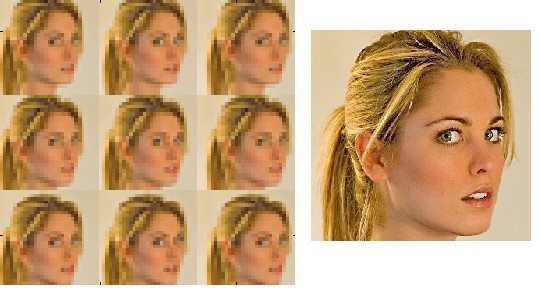
\includegraphics[width=\linewidth]{multi_sample.jpg}
    \caption{Multiple sample based approch}
    \label{fig:ms} % insert suitable label, this is used to refer to a fig from within the text
\end{figure}

\subsection{Interpolation based approach}
Interpolation-based SR algorithms construct a HR image by projecting all the acquired LR images to a reference image. All the information available from each image is then fused together, due to the fact that each LR image provides an amount of additional information about the scene, and finally a deblurring process is applied to the obtained image. 

\subsection{Frequency-domain-based approach}
A major class of multi-frames SR methods utilizes a frequency domain formulation of the SR problem. The main principle is that clues ab out high frequencies are spread across the multiple LR images in form of aliased spectral frequencies. The first frequency-domain SR method can b e credited to Tsai and Huang [8], who considered SR reconstruction from noise-free LR images. They proposed of first transform the LR image data into the Discrete Fourier Transform (DFT) domain, and then combine them according to the relationship between the aliased DFT coeffcients of the observed LR images. The approach is based on the following principles:

1. The shifting prop erty of the Fourier transform
2. The aliasing relationship b etween the continuous Fourier transform (CFT) and the DFT of observed LR images
3. The assumption that an original HR image is band-limited.

\section{Proposed System}

\begin{figure}[htb]
    \centering
    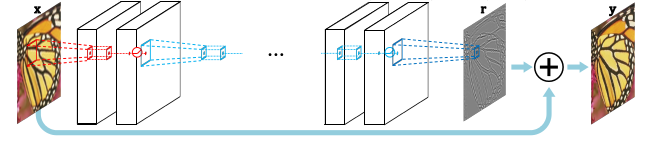
\includegraphics[width=\linewidth]{acc.png}
    \caption{Accurate Image Super Resolution}
    \label{fig:acc} % insert suitable label, this is used to refer to a fig from within the text
\end{figure}

We propose a novel super resolution method using neural networks to learn feature representations of images and then recreate enhanced versions of the image using these representations. While there are several neural networks based approaches already in place we attempt to use capsule networks to learn feature representations instead of convolutional neural networks. Capsule networks have been shown to produce slightly better results than the current goto choice of convolutional neural networks.

\begin{figure}[htb]
    \centering
    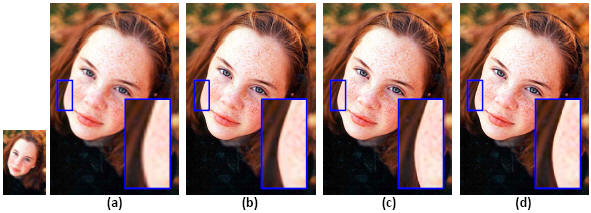
\includegraphics[width=\linewidth]{sr2.jpg}
    \caption{Better edge correction}
    \label{fig:sr2} % insert suitable label, this is used to refer to a fig from within the text
\end{figure}

Feature Extraction
In the previous Deep Learning - based methods, an upsampled image was often used as their input . In these models, the super resolution networks can be pixel - wise and its implementation becomes easier. However, they have 20 - 30 CNN layers in total and heavy computation is required for each up - sampled pixel. Furthermore, extracting features of up - sampled pixel is redundant , especially in the case of a scale factor of 3 or more. We use an original image as an input of our model so that the network can grasp the features efficiently. We also optimize the number of filters of each CNN layer and send those features directly to the image reconstruction network via skip connections.

\begin{figure}[htb]
    \centering
    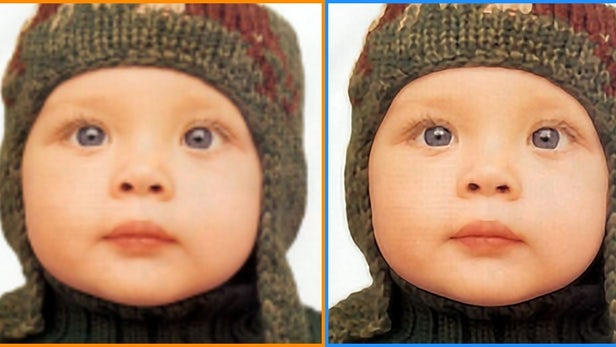
\includegraphics[width=\linewidth]{sr1.jpg}
    \caption{Blur correction}
    \label{fig:sr1} % insert suitable label, this is used to refer to a fig from within the text
\end{figure}

We also attempt to use capsule networks in place of convolutional neural networks to extract features. This should theoretically improve the feature extraction process since it has been shown that capsule networks are an improvement over conventional CNN networks.

\begin{figure}[htb]
    \centering
    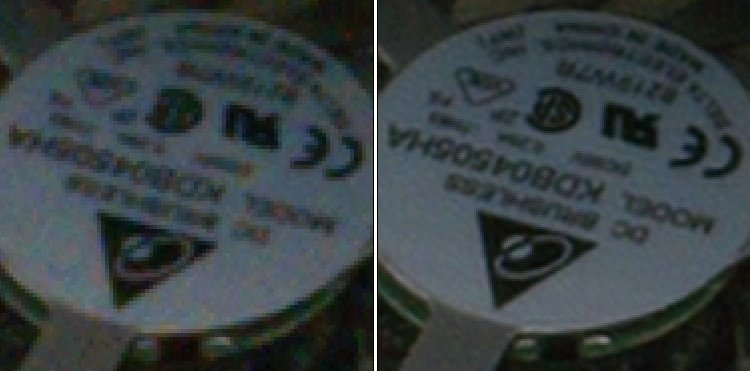
\includegraphics[width=\linewidth]{sr5.jpg}
    \caption{Better edge correction}
    \label{fig:sr5} % insert suitable label, this is used to refer to a fig from within the text
\end{figure}

Image Detail Reconstruction
In the case of data up - sampling, the transposed convolutional layer ( also known as a deconvolution layer ) proposed by Matthew D. Zeiler is typically used. T he t ransposed convolutional layer can learn up - sampling kernels, however, the process is similar to the usual convolutional layer and the reconstruction ability is limited. To obtain a better reconstruction performance, the transposed convolutional layers need to be stacked deeply , which means the process needs heavy computation. So we propose a parallelized CNN structure like the Network in Network, which usually consists of one (or more) 1x1 CNN(s). Remarkably, the 1x1 CNN layer 
